\chapter{Analiza wymagań}
\section{Założenia ogólne}
% TO DO: tutaj jeszcze tryb niedokonany - planujemy, co ma być wykonane
%        musiałem sporo przeredagować w tym rodziale, zmieniając jego układ, bo było bardzo dużo powtórzeń.

Przystępując do realizacji projektu założono, że budowana platforma będzie oferować użytkownikom szeroki wachlarz funkcji, umożliwiając im nie tylko naukę, ale także interakcję z rzeczywistymi danymi blockchainowymi. Zakres tych interakcji opisano w punktach poniżej.
\begin{enumerate}[labelwidth=1em]
\item \textbf{Sprawdzanie danych z blockchainów}: użytkownicy będą mogli przeglądać aktualne informacje o transakcjach, stanie kont i opłatach w wybranych blockchainach. Dzięki integracji z Alchemy, platforma będzie zapewniała bezpośredni dostęp do danych blockchainowych w czasie rzeczywistym. 
\item \textbf{Symulacja transakcji na blockchainie Solana}: platforma umożliwi użytkownikom przeprowadzenie symulowanych transakcji, co pozwoli na lepsze zrozumienie mechanizmów przesyłania środków bez ryzyka utraty realnych środków. 
\item \textbf{Przewidywanie cen kryptowalut}: z wykorzystaniem modeli sztucznej inteligencji użytkownicy będą mogli uzyskać prognozy dotyczące cen kryptowalut, co pomoże im w podejmowaniu decyzji inwestycyjnych. 
\item \textbf{Dostęp do materiałów edukacyjnych}: platforma będzie zawierać linki do kursów wideo, artykułów oraz innych materiałów edukacyjnych, które pozwolą użytkownikom poszerzać wiedzę na temat technologii blockchain. 
\item \textbf{Konwersja walut i kryptowalut}: funkcja konwertera ułatwi przeliczenia pomiędzy walutami tradycyjnymi a kryptowalutami, co jest istotne dla inwestorów. 
\end{enumerate}

Platforma będzie oferowała możliwość \textbf{wyboru konkretnego blockchaina do analiz i operacji}, czym różnić się będzie od istniejących serwisów, takich jak Etherscan (skoncentrowanego na Ethereum) czy Solscan (dedykowanego Solanie). Dzięki integracji z API użytkownicy będą mieli dostęp do bieżących danych o transakcjach i stanie blockchainów, co zwiększy wartość informacyjną platformy i pozwoli na podejmowanie bardziej świadomych decyzji inwestycyjnych.

Pod względem funkcjonalnym aplikacja musi umożliwiać zarządzanie użytkownikami, w tym rejestrację i logowanie za pomocą bezpiecznego mechanizmu autoryzacji opartego na OAuth2 i tokenach JWT. Użytkownicy muszą mieć możliwość przeglądania szczegółowych danych blockchainowych, takich jak transakcje, bloki i konta na blockchainach Bitcoin, Ethereum i Solana. System powinien także umożliwiać dynamiczne wyszukiwanie tych danych za pomocą zapytań REST, które frontend przesyła do backendu.

Kolejnym wymaganiem jest obsługa kryptowalut, obejmująca prezentację kategorii kryptowalut, danych historycznych oraz informacji o rynku globalnym, takich jak wskaźnik strachu i chciwości. Użytkownicy powinni mieć dostęp do danych związanych z NFT, w tym szczegółowych informacji o kolekcjach i tokenach oraz ich statystykach. System musi również umożliwiać realizację operacji blockchainowych, takich jak symulacje transakcji czy airdropy, które są wykonywane za pomocą dedykowanych skryptów Node.js.

Oprócz funkcji użytkowych system musi zapewniać przewidywanie cen kryptowalut dzięki integracji z modelem AI. Model ten będzie analizować dane historyczne i bieżące, generując prognozy, które będą udostępniane użytkownikom w aplikacji.

Pod względem niefunkcjonalnym aplikacja musi być wydajna, obsługując wiele równoczesnych zapytań REST bez znaczącego spadku wydajności. Dynamiczne pobieranie danych blockchainowych z zewnętrznych API, takich jak Etherscan czy CoinMarketCap, musi odbywać się w czasie rzeczywistym z minimalnym opóźnieniem. System musi być skalowalny.

\subsection{Zarys architektury}\label{subsec:ZarysArchitektury}
Architektura budowanej platformy ma być wielowarstwowa, z wyróżnionymi dwoma głównymi elementami: backendem i frontendem. 
Zarys architektury tej aplikacji pokazano na rysunku~\ref{fig:ZarysyArchitekturySystemu}.
\begin{figure}[htb]
    \centering
    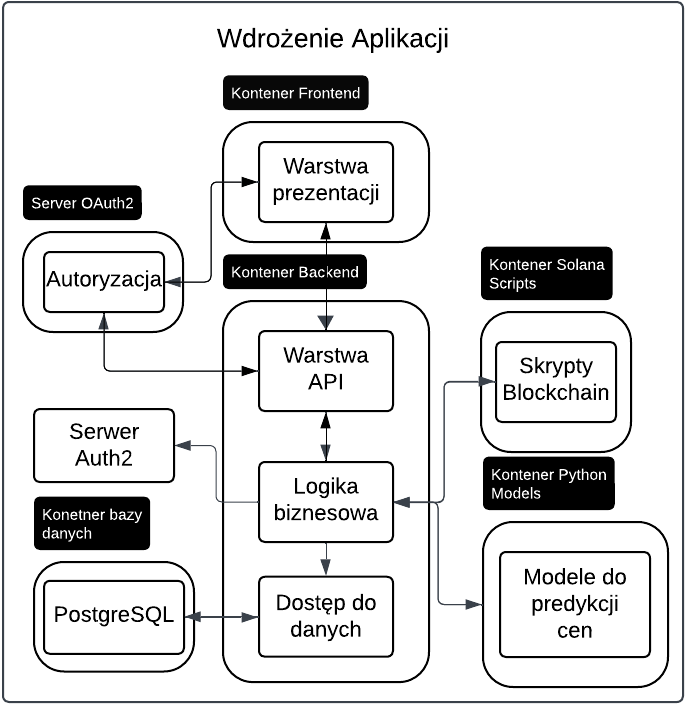
\includegraphics[width=0.9\linewidth]{Diagram.png}
    \caption{Zarysy architektury systemu}
    \label{fig:ZarysyArchitekturySystemu}
\end{figure}
Każdy komponent działać ma jako osobny moduł, uruchamiany w odrębnym kontenerze Docker, co zapewnić ma izolację środowisk oraz łatwość wdrażania i utrzymania. Komunikacja między frontendem a backendem odbywać się ma za pomocą protokołu REST, z odpowiedziami zwracanymi w formacie JSON, w postaci obiektów \texttt{ResponseEntity}, co ułatwi integrację i zapewni spójność przesyłanych danych.

Bezpieczeństwo aplikacji jest priorytetem. Wszystkie dane przesyłane między frontendem a backendem muszą być zabezpieczone za pomocą szyfrowania HTTPS, a tokeny JWT muszą być przechowywane w sposób bezpieczny w przeglądarce użytkownika. System musi być odporny na ataki oraz zapewniać ochronę przed nieautoryzowanym dostępem.

Backend, pełniący rolę centralnego punktu przetwarzania danych, zostanie zaimplementowany w Spring Boot 3 z użyciem Javy 21. Do zarządzania danymi użytkowników oraz NFT w bazie PostgreSQL wykorzystany zostanie \texttt{CrudRepository} ze Spring Data JPA. Informacje blockchainowe, takie jak transakcje i dane tokenów, będą pobierane w czasie rzeczywistym z API dostawców, takich jak Etherscan i CoinMarketCap (zakłada się możliwość zamockowania tych API do celów testowania). Backend dodatkowo wykorzystany zostanie Node.js do realizacji zaawansowanych operacji blockchainowych, w tym symulacji transakcji oraz airdropów.

Frontend, zbudowany w React, działać ma jako aplikacja wielostronicowa MPA (ang.~\emph{Multi-Page Application}). Komunikację z backendem zapewnić ma użycie biblioteki \texttt{axios}. Autoryzacja użytkowników zostanie realizowana za pomocą tokenów JWT przechowywanych w \texttt{localStorage}, co zapewni bezpieczeństwo sesji oraz ochronę komunikacji między komponentami.

System musi być również łatwy w utrzymaniu. Kod aplikacji musi być zgodny z najlepszymi praktykami programistycznymi. Planowane jest wdrożenie pipeline’u CI/CD do automatyzacji procesu budowy, testowania i wdrażania.

% TO DO: tutaj jeszcze tryb niedokonany - planujemy, co ma być wykonane

\section{Analiza wymagań}
Na podstawie założeń ogólnych sformułowano wymagania szczegółowe. Zestawiono je poniżej w kolejnych podrozdziałach. Stanowią one uzupełnienie do opisanych już wymagań. 
\subsection{Wymagania funkcjonalne}
Wymagania funkcjonalne systemu zostały podzielone na grupy w zależności od ich domeny zastosowania. Poniżej przedstawiono szczegóły każdej z tych grup.

\subsubsection{Kategorie i dane rynkowe}
\begin{itemize}
\item \textbf{Category} -- reprezentuje kategorię kryptowalut (np.\ DeFi, NFT), z jej nazwą i opcjonalnym opisem. System powinien umożliwiać wyświetlanie kategorii kryptowalut.
\item \textbf{Cryptocurrency} -- reprezentuje kryptowalutę, jej nazwę, symbol i dane rynkowe.
\item \textbf{HistoricalData} -- reprezentuje dane historyczne kryptowalut (cena, wolumen, kapitalizacja). System powinien umożliwiać przechowywanie danych historycznych i zapytanie o dane w określonym dniu w przeszłości.
\item \textbf{FearAndGreed} -- reprezentuje wskaźnik strachu i chciwości na rynku kryptowalut. System powinien umożliwiać pobieranie bieżących.
\end{itemize}

\subsubsection{Dane NFT}
\begin{itemize}
\item \textbf{Collection} -- reprezentuje kolekcję NFT, np.\ Bored Ape Yacht Club. Przechowuje nazwę, opis, liczbę tokenów w kolekcji oraz właścicieli. Powiązana z tokenami NFT.
\item \textbf{CollectionStats} -- przechowuje dane statystyczne kolekcji NFT, np. średnia cena, wolumen obrotu. Umożliwia aktualizację danych na podstawie transakcji.
\item \textbf{NFT} -- reprezentuje token NFT, w tym metadane, właściciela i historię transakcji.
\item \textbf{NFTOwner} -- przechowuje dane właścicieli NFT, np.\ ID użytkownika i adres portfela. Obsługuje powiązania między właścicielami a tokenami.
\item \textbf{NFTRarity} -- reprezentuje rzadkość tokenu NFT w skali procentowej.
\item \textbf{NFTTrait} -- przechowuje cechy tokenów NFT, np.\ kolor oczu, tło. Obsługuje mapowanie cech na tokeny.
\end{itemize}

\subsubsection{Dane blockchainowe Bitcoin}
\begin{itemize}
\item \textbf{BitcoinAccount} -- reprezentuje konto w sieci Bitcoin. Umożliwia zmapowanie surowych danych, przekształcając je w strukturę obiektową.
\item \textbf{BitcoinBlock} -- reprezentuje blok w sieci Bitcoin. Umożliwia zmapowanie surowych danych, przekształcając je w strukturę obiektową.
\item \textbf{BitcoinTransaction} -- reprezentuje transakcję w sieci Bitcoin. Umożliwia zmapowanie surowych danych, przekształcając je w strukturę obiektową.
\end{itemize}

Analogicznie będzie dla folderów Etherum oraz Solana
\subsubsection{Dodatkowe dane blockchainowe Ethereum}
\begin{itemize}
\item \textbf{Contract} -- reprezentuje inteligentny kontrakt Ethereum. Przechowuje kod, adres i ABI. Umożliwia interakcję z kontraktami i odczyt/zapis danych na blockchainie.
\end{itemize}

\subsubsection{Dodatkowe dane blockchainowe Solana}
\begin{itemize}
\item \textbf{Epoch} -- reprezentuje epokę w sieci Solana, przechowuje liczbę slotów i czas trwania. Obsługuje dynamiczne aktualizacje danych w zależności od stanu sieci.
\item \textbf{SolanaClusterNode} -- reprezentuje węzeł Solana, zawiera adres IP, status i typ roli (np. walidator). Umożliwia monitorowanie stanu węzłów klastra.
\item \textbf{SplToken} -- reprezentuje token SPL, przechowuje symbol, nazwę, liczbę dziesiętnych miejsc i adres kontraktu. Obsługuje zapytania o szczegóły tokenu i jego emisję.
\end{itemize}

\subsection{Przykłady użycia aplikacji}
Aplikacja powinna umożliwiać realizację różnych scenariuszy użytkowania, dostosowanych do potrzeb użytkowników zainteresowanych blockchainami, kryptowalutami i NFT. Poniżej przedstawiono główne przypadki użycia.

\paragraph{Przeglądanie danych blockchainowych}
Użytkownik loguje się do aplikacji, a następnie może przeglądać szczegółowe dane blockchainowe dotyczące Bitcoin, Ethereum i Solana. Na przykład może wyszukiwać adresy blockchainowe, aby uzyskać historię transakcji, saldo lub dane o blokach, takie jak wysokość i czas utworzenia. Dane są pobierane w czasie rzeczywistym z zewnętrznych API, co zapewnia aktualność informacji.

\paragraph{Analiza kryptowalut i danych rynkowych}
Użytkownik może przeglądać kategorie kryptowalut, ich dane historyczne oraz informacje o rynku globalnym, takie jak wskaźnik strachu i chciwości. Na przykład może analizować historię cen kryptowalut z ostatnich 2 lat lub uzyskać dane o wolumenie obrotu dla wybranej kategorii. Te funkcje wspierają podejmowanie decyzji inwestycyjnych.

\paragraph{Zarządzanie kolekcjami NFT}
Aplikacja pozwala przeglądać szczegóły dotyczące kolekcji NFT. Użytkownik może również wyszukiwać pojedyncze tokeny i sprawdzać ich metadane oraz historię transakcji. To przydatne dla kolekcjonerów i inwestorów NFT.

\paragraph{Symulacje transakcji blockchainowych}
Za pomocą skryptów Node.js użytkownik może symulować transakcje blockchainowe takie jak przesyłanie tokenów lub wykonywanie airdropów. Po wykonaniu operacji użytkownik dostanie informację na temat rezultatów operacji.

\paragraph{Wykorzystanie AI do przewidywania cen kryptowalut}
Model AI zintegrowany z aplikacją umożliwi prognozowanie cen kryptowalut. Użytkownik będzie wybierał datę a następnie będzie mógł zobaczyć przewidywaną cenę Bitcoina, Etheru i Sol. Wyniki są prezentowane w formie pojedyńczej wartości, co wspiera podejmowanie decyzji inwestycyjnych.

\paragraph{Dynamiczne przetwarzanie danych blockchainowych}
Aplikacja pozwala uzyskać dane blockchainowe w czasie rzeczywistym dzięki dynamicznym połączeniom z API dostawców. Użytkownik może np. przeglądać najnowsze transakcje w sieci Solana lub analizować szczegóły tokenów ERC-20 na Ethereum. Funkcjonalność ta jest kluczowa dla osób potrzebujących aktualnych danych.

\subsection{Wymagania niefunkcjonalne}
Aplikacja powinna być zaprojektowana tak, aby spełnić wymagania co do jej wydajność, skalowalność, bezpieczeństwo oraz łatwość utrzymania zdefiniowane poniżej.

\paragraph{Wydajność}
Backend musi obsługiwać co najmniej 100 równoczesnych zapytań REST bez znaczącego spadku wydajności. Dynamiczne pobieranie danych blockchainowych z zewnętrznych API musi odbywać się w czasie rzeczywistym z minimalnym opóźnieniem, aby zapewnić użytkownikom aktualne informacje.

\paragraph{Skalowalność}
System musi być skalowalny i dostosowany do zwiększającej się liczby użytkowników. Planowane wdrożenie w chmurze AWS z wykorzystaniem Elastic Load Balancer (ELB) umożliwi równoważenie obciążenia oraz dynamiczne zarządzanie zasobami.

\paragraph{Bezpieczeństwo}
Wszystkie dane przesyłane między frontendem a backendem muszą być zabezpieczone szyfrowaniem HTTPS. Tokeny JWT muszą być bezpiecznie przechowywane w \texttt{localStorage} i weryfikowane przez backend przy każdym zapytaniu. System musi być odporny na ataki CSRF i XSS, a dane użytkowników muszą być chronione przed nieautoryzowanym dostępem.

\paragraph{Niezawodność}
Aplikacja musi zapewniać 99,9\% dostępności, co zostanie osiągnięte dzięki konteneryzacji oraz planowanemu wdrożeniu na AWS. Mechanizmy monitorowania i powiadamiania o błędach lub awariach muszą zapewnić szybką reakcję na problemy.

\paragraph{Elastyczność}
Architektura aplikacji musi umożliwiać łatwe dodawanie nowych funkcjonalności, takich jak obsługa kolejnych blockchainów czy wdrażanie modeli analitycznych AI. Modularna budowa, w której każdy komponent działa jako niezależny kontener Docker, wspiera tę elastyczność.

\paragraph{Łatwość utrzymania}
Kod aplikacji musi być zgodny z najlepszymi praktykami, w tym zasadami SOLID i wzorcami projektowymi, co zapewni jego łatwą rozbudowę i utrzymanie. Planowane wdrożenie pipeline'u CI/CD usprawni procesy budowy, testowania i wdrażania.

\paragraph{Zgodność technologiczna}
Aplikacja musi działać w środowisku obsługującym Dockera. Backend opiera się na Javie 21 i Spring Boot 3, a frontend został zaimplementowany w React, co zapewnia kompatybilność z nowoczesnymi przeglądarkami, takimi jak Chrome, Firefox i Safari.


\section{Podsumowanie}

W rozdziale przedstawiono analizę wymagań, od ogólnych założeń po szczegóły dotyczące zarówno planowanych funkcji systemu, jak i aspektów technicznych związanych z ich implementacją. Opisano kluczowe funkcje platformy, takie jak przeglądanie danych blockchainowych, zarządzanie kryptowalutami i NFT, symulacje transakcji oraz przewidywanie cen z wykorzystaniem modeli AI. Wyróżnikiem aplikacji jest integracja z zewnętrznymi API blockchainowymi, co umożliwia dynamiczne pobieranie danych w czasie rzeczywistym i oferowanie unikalnych funkcji dla użytkowników.

Architektura systemu opiera się na modularnym podejściu, z wyraźnym podziałem na frontend i backend, wspieranych przez skrypty Node.js i Python oraz bazę danych PostgreSQL. Dzięki konteneryzacji każdy komponent działa w izolowanym środowisku, co zapewnia elastyczność, skalowalność i łatwość utrzymania. Interakcje między komponentami odbywają się za pomocą protokołu REST, z uwierzytelnieniem opartym na OAuth2 i tokenach JWT, co gwarantuje bezpieczeństwo komunikacji.

Wymagania niefunkcjonalne aplikacji koncentrują się na wydajności, skalowalności oraz niezawodności. Planowane wdrożenie w chmurze AWS z wykorzystaniem Elastic Load Balancer (ELB) pozwoli na dynamiczne zarządzanie zasobami i równoważenie obciążenia. Dodatkowo, zastosowanie pipeline’u CI/CD usprawni procesy związane z utrzymaniem i rozwojem systemu, zapewniając jego długoterminową stabilność.

Podsumowując, aplikacja jest wszechstronnym narzędziem, które dzięki modularnej architekturze i zaawansowanym funkcjom sprosta wymaganiom zarówno inwestorów, jak i entuzjastów blockchainów. System oferuje wysoką elastyczność i bezpieczeństwo, co czyni go odpowiednim rozwiązaniem dla dynamicznie zmieniającego się rynku kryptowalut i technologii blockchain.

